\documentclass[12pt, titlepage]{article}

\usepackage{booktabs}
\usepackage{tabularx}
\usepackage{graphicx}
\usepackage{fancyhdr}
\usepackage[margin=1in]{geometry}
\usepackage{enumerate}
\usepackage[utf8]{inputenc}
\usepackage{ulem}
\usepackage{placeins}
\usepackage{comment}
\usepackage{float}
\usepackage{hyperref}
\restylefloat{table}

\usepackage[round]{natbib}
\pagestyle{plain}  
\renewcommand\headrulewidth{0.4pt}

\renewcommand\footrulewidth{0.4pt}

\newcounter{benum}
\newcommand{\bethebenum}{BE\thebenum}
\newcommand{\beref}[1]{BE\ref{#1}}

\newcounter{reqnum}
\newcommand{\reqthereqnum}{\textbf{Req. \#}: \thereqnum}
\newcommand{\reqref}[1]{Req. \#: \ref{#1}}

\newenvironment{boxed}
    {\begin{center}
    \begin{tabular}{|p{0.9\textwidth}|}
    \hline\\
    }
    { 
    \\\\\hline
    \end{tabular} 
    \end{center}
    }

%% Comments

\usepackage{color}

\newif\ifcomments\commentstrue %displays comments
%\newif\ifcomments\commentsfalse %so that comments do not display

\ifcomments
\newcommand{\authornote}[3]{\textcolor{#1}{[#3 ---#2]}}
\newcommand{\todo}[1]{\textcolor{red}{[TODO: #1]}}
\else
\newcommand{\authornote}[3]{}
\newcommand{\todo}[1]{}
\fi

\newcommand{\wss}[1]{\authornote{blue}{SS}{#1}} 
\newcommand{\plt}[1]{\authornote{magenta}{TPLT}{#1}} %For explanation of the template
\newcommand{\an}[1]{\authornote{cyan}{Author}{#1}}

%% Common Parts

\newcommand{\progname}{Software Engineering} % PUT YOUR PROGRAM NAME HERE
\newcommand{\authname}{Team 17, Track a Trace
\\ Zabrain Ali
\\ Linqi Jiang
\\ Jasper Leung
\\ Mike Li 
\\ Mengtong Shi
\\ Hongzhao Tan
} % AUTHOR NAMES                  

\usepackage{hyperref}
    \hypersetup{colorlinks=true, linkcolor=blue, citecolor=blue, filecolor=blue,
                urlcolor=blue, unicode=false}
    \urlstyle{same}
                                


\begin{document}

\title{Software Requirements Specification for \progname: PyERT} 
\author{\authname}
\date{November 14, 2022}
	
\maketitle

\pagenumbering{roman}
\tableofcontents
\listoftables
\listoffigures

\begin{table}[H]
\caption{\bf Revision History}
\begin{tabularx}{\textwidth}{p{3cm}p{2cm}X}
\toprule {\bf Date} & {\bf Version} & {\bf Notes}\\
\midrule
05/10/2022 & 1.0 & Initial Software Requirements Specification\\
02/11/2022 & 1.1 & Modified Functional Requirements and Naming Conventions\\
14/11/2022 & 1.2 & Modified Functional Requirements\\
\bottomrule
\end{tabularx}
\end{table}

\newpage

\pagenumbering{arabic}

This document describes the requirements for PyERT. The template for the Software Requirements Specification (SRS) is a subset of the Volere template~\citep{RobertsonAndRobertson2012} with sections for System Description and Reflection added into it.
% If you make further modifications to the template, you should explicitly state what modifications were made.

\section{Project Drivers}

\subsection{Naming Conventions and Terminology}
\begin{table}[h]
\centering
\begin{tabular}{|c|p{10cm}|}
 \hline
 {\bf Acronym/Abbreviation} & {\bf Definition} \\
 \hline
 GIS & Geographic Information System \\
 \hline
 GERT & GIS-based Episode Reconstruction Toolkit  \\ 
\hline
 ArcGIS & A licensed GIS service used by GERT for data processing \\
 \hline
 PyERT & Python-based Episode Reconstruction Toolkit  \\ 
 \hline
 Req. & Requirement  \\
 \hline
 NFR & Non-Functional Requirement  \\
 \hline 
 CSV & Comma Separated Values \\
 \hline
 GPS & Global Positioning System \\
 \hline
 TUD & Time Use Diary:  Survey data containing a chronological sequence of activities that respondents did over a time period\\
 \hline
 m/s & meters per second\\
 \hline
 SHP & shapefile: A data format for spreadsheet \\ 
 \hline
 LU & Land Use \\ 
 \hline
 PAL & Potential Activity Locations \\ 
 \hline
 CI/CD & Continuous Integration / Continuous Deployment\\
 \hline
 \textcolor{red}{RCA} & \textcolor{red}{Route Choice Analysis} \\
 \hline
\end{tabular}
\caption{\bf Naming Conventions and Terminology}
\end{table}

    \subsection{The Purpose of the Project}
This project aims to re-implement the features in GERT~\citep{DALUMPINES2018121} that use ArcGIS Pro packages with
open-source packages and libraries, and remove any use of ArcGIS in the project. Using open-source packages and libraries instead of ArcGIS will make GERT tools accessible. The changes that were made to GERT when replacing ArcGIS will be documented, as having detailed documentation for the modified GERT will ensure that existing users of GERT will be able to transition from using the ArcGIS-free version easily and understand the changes made, and will also be helpful for new users. The current project structure will be modified to be more organized and readable, because most of the code for the current project is stored in a single file, making it hard to read. Organizing the code and potentially splitting up the code into separate modules would be helpful for any users trying to use the code.

\subsection{The Stakeholders}

The stakeholders of this project include The School of Earth, Environment and Society of McMaster University, the supervisor of the project, Dr. Antonio Paez, 4G06 Capstone Project course teaching assistants, and the professor, Dr. Spencer Smith. 

\subsubsection{The Client}

The clients of this project consists of The School of Earth, Environment and Society of McMaster University and the supervisor of the project, Dr. Antonio Paez. The primary concern for the clients is to see that the outcome of the project is an open-source and potentially upgraded version of the original GERT toolkit.

\subsubsection{The Customers}

The target demographic of this project is aimed at potential users who would develop projects based on GERT or refer to it, members of the school of The Earth, Environment and Society of McMaster University, and the supervisor of the project, Dr. Antonio Paez.

\subsubsection{Other Stakeholders}

There are many other stakeholders involved in this project. The development team is a major stakeholder, as they are responsible for re-implementing and upgrading the original GERT toolkit. The development team has their own desires for what the overall outcome should be, some of which include technical aspects such as efficiency, run time, organizing the structure of the project and  stylizing the code.

\subsection{Mandated Constraints}
The main mandated constraints for this project involve the due dates for project deliverables. The final version of the project must not include usage of any package or library that need a license to be accessed. As this project is based off an existing toolkit, GERT, the inputs and outputs of this project must match the inputs and outputs of GERT. As such, this project shall only accept GPS or TUD data in CSV format, and shall return only CSV or SHP files after processing the user input if there are no errors.

\subsection{Relevant Facts and Assumptions}

\subsubsection{Relevant Facts}
The goal of the original GERT toolkit is to break the limit of previously developed procedures in terms of scalability, modularity and transferability. With this effective toolkit, we can take full advantage of GPS data for the following reasons: (1) it is difficult to adopt tools developed by other researchers because of the lack of transferability, (2) the limited ability to derive more information from GPS data for lack of an integrated set of modules, and (3) high computational costs and lack of automatic procedures in dealing with large data-sets. 

\subsubsection{Assumptions}
\begin{itemize}
    \item The project assumes the users will directly run the compiled .pyc files of the source code .py files with command line in console to use the product.
\end{itemize}

\section{System Description}

\subsection{System Context}

\begin{figure}[!htbp]
    \centering
    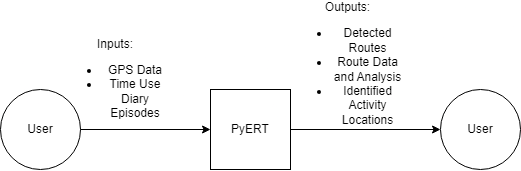
\includegraphics[scale=0.75]{contextdiagram.png}
    \caption{\bf Context Diagram}
\end{figure}

\begin{itemize}
\item User responsibilities: 
    \begin{itemize}
        \item Input a data-set containing GPS information in CSV format (mandatory) and TUD episodes in CSV format (optional).
        \item Ensure the general format of the input data is correct.
    \end{itemize}
    
    \item PyERT responsibilities: 
        \begin{itemize}
        \item Filter faulty TUD episodes and GPS data.
        \item Return detected routes, generated data for those routes, and identified potential activity locations in the correct format.
        \end{itemize}
\end{itemize}

\subsection{Normal Operation}
This program is used to process geographical data. Users will use the program on a computer, which allows them to view and save the processed data. Users will then be able utilize the processed data in any manner they choose.
\subsection{Behaviour Overview}
The system requires user input in order to begin processing and returning data. The program will accept geographical data in the form of a CSV file. The user must provide a CSV file containing GPS points, and can optionally provide a CSV file with TUD data and SHP files with data on LU and PAL. If no TUD CSV file is provided, the program will use its own generated data during processing. If a TUD CSV file is provided, the program will use the data in the provided file during processing. The program will filter faulty GPS points, and will return processed data on route choices in SHP and CSV files. Activity location data will also be returned with LU and PAL data appended if they were provided, in the form of a SHP file.
\subsection{Undesired Event Handling}
If an undesired event occurs during operation of the program, the program shall enter an error state. The program shall not process any data in this state to ensure corrupted or incorrect data is not used, and that it does not corrupt the user's inputted data. A reason for the error will be displayed so that the user understands the undesired event and potentially avoids it in the future. The program will need to be run again and will require the user to re-input their data, to ensure the undesired event does not affect the programs results.
\subsection{User Characteristics}
\begin{itemize}
    \item The end user of PyERT should have an understanding of basic geographic concepts (GPS, latitude, longitude, etc.).
    \item The end user of PyERT should know the input formats of the GPS data-sets and TUD Episodes.
    \item The end user of PyERT should understand the relevance of the GPS data-sets and Time Use Diaries being input into the program.
    \item The end user of PyERT should have an understanding of the Route Data and activity analysis provided by PyERT.
\end{itemize}
\section{Functional Requirements}
\subsection{The Scope of the Work and the Product}

\subsubsection{The Context of the Work}
The plan for the project is to re-implement the features of the original GERT toolkit, where packages require an ArcGIS Pro license, and implement it with open-source packages and libraries so that the toolkit can be independent from ArcGIS Pro. The re-implemented version of the toolkit (PyERT) should inherit all functionalities of the original GERT toolkit. In addition, the structure of the implementation of the toolkit shall be reorganized into modules that are more readable and understandable for users who are trying to access the code.

\subsubsection{Work Partitioning}

%\begin{comment}
\begin{table}[H]
\begin{tabular}{|p{5cm}|p{5cm}|p{5cm}|}
\hline
{\bf Event ID} & {\bf Event Name} & {\bf Summary} \\ 
\hline
 \refstepcounter{benum} \bethebenum \label{BE1} & Matching GPS Data Point to Network with TUD Episodes Input & User executes PyERT toolkit using command line in console with input GPS data and TUD Episodes. \\ 
\hline
 \refstepcounter{benum} \bethebenum \label{BE2} & Matching GPS Data Point to Network without TUD Episodes Inputs & User executes PyERT toolkit using command line in console with input GPS data only. \\ 
\hline
 \refstepcounter{benum} \bethebenum \label{BE3} & Invalid Input from User & User executes PyERT toolkit using command line in console with invalid input. \\
\hline
\end{tabular}
\caption{\bf Work Partitioning Part 1}
\end{table}

\begin{table}[H]
\begin{tabular}{|p{5cm}|p{5cm}|p{5cm}|}
\hline
{\bf Event ID} & {\bf Input} & {\bf Output} \\ 
\hline
\beref{BE1} & User's GPS data, TUD Episodes in CSV format and LU and PAL information in SHP format & Route Choice Set and Activity Locations' Information in SHP file type and RCA Variables in CSV format  \\ 
\hline
\beref{BE2} & User's GPS data in CSV format and LU and PAL information in SHP format & Route Choice Set and Activity Locations' Information in SHP file type and RCA Variables in CSV format \\ 
\hline
\beref{BE3} & User's data not in CSV format or user's CSV file but with data that cannot be processed by PyERT & Descriptive error message shall be shown to the user \\ 
\hline
\end{tabular}
\caption{\bf Work Partitioning Part 2}
\end{table}

\newpage

\subsubsection{Individual Product Use Cases}
\begin{figure}[!htbp]
    \centering
    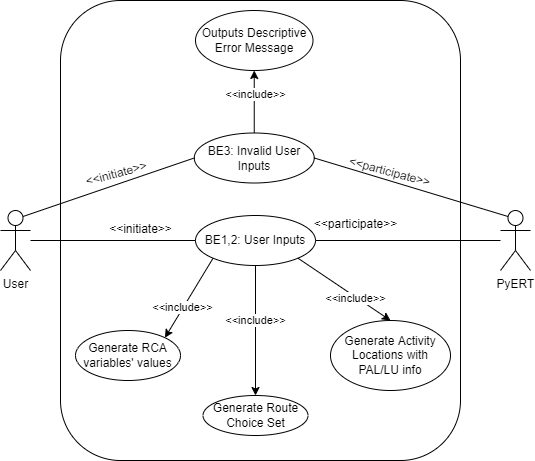
\includegraphics[scale=0.75]{Use_Case_Diagram.png}
    \caption{\bf Use Case Diagram}
\end{figure}

\subsection{Functional Requirements}

\begin{boxed}
\begin{tabular}{l r r}
\refstepcounter{reqnum} \reqthereqnum \label{Req1} & {\bf Req. Type}: &  Functional\\
\end{tabular}
\newline
\begin{tabular}{l p{11.5cm}}
    {\bf Description:} & The product shall be able to read and generate CSV and SHP files.  \\
    {\bf Rationale:} & Since the product is a re-implemented version of the GERT toolkit, it shall be able to take and generate the same types of files the GERT toolkit used to take and generate as its inputs and outputs respectively.\\
    {\bf Organizer:} & Software Engineer\\
    {\bf Fit Criterion:} & After the user executes the product with valid input data in CSV and SHP formats, the product will be able to read the data from the input and generate required CSV and SHP files after processing the input data.\\
\end{tabular}
\begin{tabular}{l r}
{\bf Costumer Satisfaction:} N/A &  {\bf Costumer Dissatisfaction:}  N/A\\
\end{tabular}
\begin{tabular}{l r r}
    {\bf Priority}: 1 & {\bf Dependencies}: None  & {\bf Conflicts}: None \\
\end{tabular}
\begin{tabular}{l l}
     {\bf Supporting Materials}:& 
     \beref{BE1}, \beref{BE2} \\ 
     {\bf History}: & Created October 5, 2022\\
     {\bf Plan to Complete by}: & January 6, 2023\\
\end{tabular}
\end{boxed}

\begin{boxed}
\begin{tabular}{l r r}
\refstepcounter{reqnum} \reqthereqnum \label{Req2} & {\bf Req. Type}: &  Functional\\
\end{tabular}
\newline
\begin{tabular}{l p{11.5cm}}
    {\bf Description:} & The product shall remove invalid GPS points from user's input. Invalid points include redundant points (points with the same coordinates) and outliers (with speed $\ge$ 50m/s).  \\
    {\bf Rationale:} & Since there could be some invalid GPS points in users' input GPS data which could affect the result of matching GPS points to network or the performance of the product. The requirement is needed for the product to determine and remove the invalid GPS points before actually processing them.\\
    {\bf Organizer:} & Software Engineer\\
    {\bf Fit Criterion:} & The product will remove points with the same coordinates and points that are with speed $\ge$ 50m/s. \\
\end{tabular}
\begin{tabular}{l r}
{\bf Costumer Satisfaction:} N/A &  {\bf Costumer Dissatisfaction:}  N/A\\
\end{tabular}
\begin{tabular}{l r r}
    {\bf Priority}: 2 & {\bf Dependencies}: None  & {\bf Conflicts}: None \\
\end{tabular}
\begin{tabular}{l l}
     {\bf Supporting Materials}:& 
     \beref{BE1}, \beref{BE2} \\ 
     {\bf History}: & Created October 5, 2022\\
     {\bf Plan to Complete by}: & January 12, 2023\\
\end{tabular}
\end{boxed}

\begin{boxed}
\begin{tabular}{l r r}
\refstepcounter{reqnum} \reqthereqnum \label{Req3} & {\bf Req. Type}: &  Functional\\
\end{tabular}
\newline
\begin{tabular}{l p{11.5cm}}
    {\bf Description:} & The product shall be able to divide GPS points into 24-hour trajectories and further divide the trajectories into clusters of adjacent points based on speed, distance, heading and change-in-heading thresholds.  \\
    {\bf Rationale:} & The requirement is needed since the GPS points from users' input need to be divided into clusters that represents the movement of each person-day or of even shorter time period so that the points can be further processed by the product.\\
    {\bf Organizer:} & Software Engineer\\
    {\bf Fit Criterion:} & The product will divide input GPS points into clusters of adjacent points based on predefined thresholds.\\
\end{tabular}
\begin{tabular}{l r}
{\bf Costumer Satisfaction:} N/A &  {\bf Costumer Dissatisfaction:}  N/A\\
\end{tabular}
\begin{tabular}{l r r}
    {\bf Priority}: 2 & {\bf Dependencies}: None  & {\bf Conflicts}: None \\
\end{tabular}
\begin{tabular}{l l}
     {\bf Supporting Materials}:& 
     \beref{BE1}, \beref{BE2} \\ 
     {\bf History}: & Created October 5, 2022\\
     {\bf Plan to Complete by}: & January 12, 2023\\
\end{tabular}
\end{boxed}

\begin{boxed}
\begin{tabular}{l r r}
\refstepcounter{reqnum} \reqthereqnum \label{Req4} & {\bf Req. Type}: &  Functional\\
\end{tabular}
\newline
\begin{tabular}{l p{11.5cm}}
    {\bf Description:} & The product shall tag each valid input GPS point as a stop (stationary) point or a trip (moving) point.  \\
    {\bf Rationale:} & The requirement is necessary for the product to further classify the GPS trajectories into trip (moving) and stop (stationary) segments.\\
    {\bf Organizer:} & Software Engineer\\
    {\bf Fit Criterion:} & All valid input GPS points will be tagged as a stop point or trip point after being clustered. \\
\end{tabular}
\begin{tabular}{l r}
{\bf Costumer Satisfaction:} N/A &  {\bf Costumer Dissatisfaction:}  N/A\\
\end{tabular}
\begin{tabular}{l r r}
    {\bf Priority}: 3 & {\bf Dependencies}: \reqref{Req2}, \reqref{Req3}  & {\bf Conflicts}: None \\
\end{tabular}
\begin{tabular}{l l}
     {\bf Supporting Materials}:& 
     \beref{BE1}, \beref{BE2} \\ 
     {\bf History}: & Created October 5, 2022\\
     {\bf Plan to Complete by}: & January 18, 2023\\
\end{tabular}
\end{boxed}

\begin{boxed}
\begin{tabular}{l r r}
\refstepcounter{reqnum} \reqthereqnum \label{Req5} & {\bf Req. Type}: &  Functional\\
\end{tabular}
\newline
\begin{tabular}{l p{11.5cm}}
    {\bf Description:} & The product shall partition valid GPS trajectories into segments \textcolor{red}{\sout{and classify the segments into stationary activity (stop) episodes and travel (moving) episodes}}.  \\
    {\bf Rationale:} & The requirement is needed to fully capture the valuable information from the perspective of activity analysis.\\
    {\bf Organizer:} & Software Engineer\\
    {\bf Fit Criterion:} & \textcolor{red}{\sout{Modules that can automatically capture land interest points details will be developed.}
    The product will generate partitioned segments given valid GPS trajectories.}\\
\end{tabular}
\begin{tabular}{l r}
{\bf Costumer Satisfaction:} N/A &  {\bf Costumer Dissatisfaction:}  N/A\\
\end{tabular}
\begin{tabular}{l r r}
    {\bf Priority}: 4 & {\bf Dependencies}: \reqref{Req4} & {\bf Conflicts}: None \\
\end{tabular}
\begin{tabular}{l l}
     {\bf Supporting Materials}:& 
     \beref{BE1}, \beref{BE2} \\ 
     {\bf History}: & Created October 5, 2022\\
     {\bf Plan to Complete by}: & January 24, 2023\\
\end{tabular}
\end{boxed}

\begin{boxed}
\begin{tabular}{l r r}
\refstepcounter{reqnum} \reqthereqnum \label{Req6} & {\bf Req. Type}: &  Functional\\
\end{tabular}
\newline
\begin{tabular}{l p{11.5cm}}
    {\bf Description:} & The product shall extract trip segments (sequences of GPS points in travel episode) from valid GPS trajectories.  \\
    {\bf Rationale:} & The requirement is needed to fully capture the valuable information from the perspective of activity analysis.\\
    {\bf Organizer:} & Software Engineer\\
    {\bf Fit Criterion:} & \textcolor{red}{\sout{The availability of huge GPS data and the high potential to collect more make it a necessary procedure that can automatically extract information from these data.}
    The product will extract all the trip segments if the GPS trajectories are valid.}\\
\end{tabular}
\begin{tabular}{l r}
{\bf Costumer Satisfaction:} N/A &  {\bf Costumer Dissatisfaction:}  N/A\\
\end{tabular}
\begin{tabular}{l r r}
    {\bf Priority}: 5 & {\bf Dependencies}: \reqref{Req5} & {\bf Conflicts}: None \\
\end{tabular}
\begin{tabular}{l l}
     {\bf Supporting Materials}:& 
     \beref{BE1}, \beref{BE2} \\ 
     {\bf History}: & Created October 5, 2022\\
     {\bf Plan to Complete by}: & January 31, 2023\\
\end{tabular}
\end{boxed}

\begin{boxed}
\begin{tabular}{l r r}
\refstepcounter{reqnum} \reqthereqnum \label{Req7} & {\bf Req. Type}: &  Functional\\
\end{tabular}
\newline
\begin{tabular}{l p{11.5cm}}
    {\bf Description:} & The product shall extract activity locations (GPS points in stop episode or end points of trip segments) from valid GPS trajectories.  \\
    {\bf Rationale:} & The requirement is necessary for the further process to add LU and PAL information to the stationary GPS points.\\
    {\bf Organizer:} & Software Engineer\\
    {\bf Fit Criterion:} & If the user inputs the valid GPS trajectories, the product will extract the correct activity locations for the user.\\
\end{tabular}
\begin{tabular}{l r}
{\bf Costumer Satisfaction:} N/A &  {\bf Costumer Dissatisfaction:}  N/A\\
\end{tabular}
\begin{tabular}{l r r}
    {\bf Priority}: 5 & {\bf Dependencies}: \reqref{Req5}  & {\bf Conflicts}: None \\
\end{tabular}
\begin{tabular}{l l}
     {\bf Supporting Materials}:& 
     \beref{BE1}, \beref{BE2} \\ 
     {\bf History}: & Created October 5, 2022\\
     {\bf Plan to Complete by}: & January 31, 2023\\
\end{tabular}
\end{boxed}

\begin{boxed}
\begin{tabular}{l r r}
\refstepcounter{reqnum} \reqthereqnum \label{Req8} & {\bf Req. Type}: &  Functional\\
\end{tabular}
\newline
\begin{tabular}{l p{11.5cm}}
    {\bf Description:} & The product shall generate \textcolor{red}{\sout{alternative} one} route\textcolor{red}{\sout{s}} for each trip segments in SHP format with digital road/pedestrian networks \textcolor{red}{\sout{and assign values to RCA variables for each of the alternative routes in CSV format based on road network attributes that are provided}}.  \\
    {\bf Rationale:} & \textcolor{red}{\sout{Both are} SHP is a} cross-platform data format\textcolor{red}{\sout{s}} for \textcolor{red}{\sout{spreadsheet and}} GIS applications\textcolor{red}{\sout{, respectively};} thus, it makes it easy to manipulate GERT’s outputs in other applications. \\
    {\bf Organizer:} & Software Engineer\\
    {\bf Fit Criterion:} &  \textcolor{red}{\sout{GERT is designed to work on minimal inputs with generic variables such as location coordinates and time stamps. This feature allows implementation in environments without additional information aside from GPS data.} Given trip segments in SHP format with digital road/pedestrian networks, the product will generate alternative routes.}\\
\end{tabular}
\begin{tabular}{l r}
{\bf Costumer Satisfaction:} N/A &  {\bf Costumer Dissatisfaction:}  N/A\\
\end{tabular}
\begin{tabular}{l r r}
    {\bf Priority}: 6 & {\bf Dependencies}:  \reqref{Req6} & {\bf Conflicts}: None \\
\end{tabular}
\begin{tabular}{l l}
     {\bf Supporting Materials}:& 
     \beref{BE1}, \beref{BE2} \\ 
     {\bf History}: & Created October 5, 2022\\
     {\bf Plan to Complete by}: & February 6, 2023\\
\end{tabular}
\end{boxed}

\begin{boxed}
\begin{tabular}{l r r}
\refstepcounter{reqnum} \reqthereqnum \label{Req9} & {\bf Req. Type}: &  Functional\\
\end{tabular}
\newline
\begin{tabular}{l p{11.5cm}}
    {\bf Description:} & The product shall generate SHP files for extracted activity locations with additional information about them when the information is available in given spatial data such as LU and PAL data in user's input.  \\
    {\bf Rationale:} & SHP is a standard format for spatial data across different GIS platforms,the outputs can be used to visualize activity episodes in a GIS or can be used as inputs to spatial analysis and modeling outside of GERT.\\
    {\bf Organizer:} & Software Engineer\\
    {\bf Fit Criterion:} & The file can be generated from spatial data such as land use and potential activity locations (PAL) using overlay analysis functions in GIS. PAL refers to points of interest that indicate the locations of government offices, shopping destinations, banks, and so on.\\
\end{tabular}
\begin{tabular}{l r}
{\bf Costumer Satisfaction:} N/A &  {\bf Costumer Dissatisfaction:}  N/A\\
\end{tabular}
\begin{tabular}{l r r}
    {\bf Priority}: 6 & {\bf Dependencies}:  \reqref{Req7}  & {\bf Conflicts}: None \\
\end{tabular}
\begin{tabular}{l l}
     {\bf Supporting Materials}:& 
     \beref{BE1}, \beref{BE2} \\ 
     {\bf History}: & Created October 5, 2022\\
     {\bf Plan to Complete by}: & February 6, 2023\\
\end{tabular}
\end{boxed}

\begin{boxed}
\begin{tabular}{l r r}
\refstepcounter{reqnum} \reqthereqnum \label{Req10} & {\bf Req. Type}: &  Functional\\
\end{tabular}
\newline
\begin{tabular}{l p{11.5cm}}
     {\bf Description:} & The product shall \textcolor{red}{\sout{handle run-time errors and}} generate descriptive error messages to the user when the user's input is invalid (not in CSV and SHP format, or data input cannot be processed by the product).  \\
    {\bf Rationale:} & It is necessary for the product to help the user understand the cause of error.\\
    {\bf Organizer:} & Software Engineer\\
    {\bf Fit Criterion:} & If there is a run-time error occurred, a descriptive message about the error will be shown to the user.\\
\end{tabular}
\begin{tabular}{l r}
{\bf Costumer Satisfaction:} N/A &  {\bf Costumer Dissatisfaction:}  N/A\\
\end{tabular}
\begin{tabular}{l r r}
    {\bf Priority}: 1 & {\bf Dependencies}: None  & {\bf Conflicts}: None \\
\end{tabular}
\begin{tabular}{l l}
     {\bf Supporting Materials}:& 
     \beref{BE3} \\ 
     {\bf History}: & Created October 5, 2022\\
     {\bf Plan to Complete by}: & January 6, 2023\\
\end{tabular}
\end{boxed}

\textcolor{red}{
\begin{boxed}
\begin{tabular}{l r r}
\refstepcounter{reqnum} \reqthereqnum \label{Req11} & {\bf Req. Type}: &  Functional\\
\end{tabular}
\newline
\begin{tabular}{l p{11.5cm}}
    {\bf Description:} & The product shall classify the segments partitioned from GPS trajectories into stationary activity (stop) episodes and travel (moving) episodes.  \\
    {\bf Rationale:} & The requirement is needed to fully capture the valuable information from the perspective of activity analysis.\\
    {\bf Organizer:} & Software Engineer\\
    {\bf Fit Criterion:} & The segments will be classified as stationary activity (stop) episodes or travel (moving) episodes.\\
\end{tabular}
\begin{tabular}{l r}
{\bf Costumer Satisfaction:} N/A &  {\bf Costumer Dissatisfaction:}  N/A\\
\end{tabular}
\begin{tabular}{l r r}
    {\bf Priority}: 4 & {\bf Dependencies}: \reqref{Req4} & {\bf Conflicts}: None \\
\end{tabular}
\begin{tabular}{l l}
     {\bf Supporting Materials}:& 
     \beref{BE1}, \beref{BE2} \\ 
     {\bf History}: & Created October 5, 2022\\
     {\bf Plan to Complete by}: & January 24, 2023\\
\end{tabular}
\end{boxed}
}

\textcolor{red}{
\begin{boxed}
\begin{tabular}{l r r}
\refstepcounter{reqnum} \reqthereqnum \label{Req12} & {\bf Req. Type}: &  Functional\\
\end{tabular}
\newline
\begin{tabular}{l p{11.5cm}}
    {\bf Description:} & The product shall assign values to RCA variables in CSV format for each of the alternative routes generated based on the provided road network attributes.  \\
    {\bf Rationale:} & CSV is a cross-platform data format for spreadsheet applications; thus, it makes it easy to manipulate GERT’s outputs in other applications. \\
    {\bf Organizer:} & Software Engineer\\
    {\bf Fit Criterion:} & Given the generated alternative routes, the product will assign the corresponding values to RCA variables in CSV format.\\
\end{tabular}
\begin{tabular}{l r}
{\bf Costumer Satisfaction:} N/A &  {\bf Costumer Dissatisfaction:}  N/A\\
\end{tabular}
\begin{tabular}{l r r}
    {\bf Priority}: 6 & {\bf Dependencies}:  \reqref{Req6} & {\bf Conflicts}: None \\
\end{tabular}
\begin{tabular}{l l}
     {\bf Supporting Materials}:& 
     \beref{BE1}, \beref{BE2} \\ 
     {\bf History}: & Created October 5, 2022\\
     {\bf Plan to Complete by}: & February 6, 2023\\
\end{tabular}
\end{boxed}
}

\section{Non-functional Requirements}

\subsection{Look and Feel Requirements}
\begin{enumerate}[{LF}1. ] 
    \item \label{LF1} The interface of the program should be easy to follow, and clearly specify the user input.
    \begin{itemize} 
        \item Rationale: A clear interface ensures that the program is easy to use and navigate through.
        \item Fit Criterion: At least 90\% of the test users for the program will say that the program's interface is clear and concise.
    \end{itemize}  
    \item \label{LF2} The program shall give visual indication stating what stage the program is in.
    \begin{itemize} 
        \item Rationale: Since the program output is not instant, there needs to be a visual indication of what stage of processing the program is in, to confirm to the user that it is running properly.
        \item Fit Criterion: At least 90\% of the test users for the program shall report that the visual indicators displaying the program progress was helpful in determining what was going on within the program.
    \end{itemize}
\end{enumerate}

\subsection{Usability and Humanity Requirements}
\begin{enumerate}[{UH}1. ]
\item \label{UH1} The program shall be easy to install.
    \begin{itemize}
        \item Fit Criterion: 90\% of users with no programming experience must be able to install the program by themselves.
\end{itemize}
\item \label{UH2} The program shall be easy to use.
    \begin{itemize}
        \item Fit Criterion: 95\% of users must be able to use the program and process data by themselves.
\end{itemize}
\item \label{UH3} The program shall be able to display instructions on how to use it.
    \begin{itemize} 
        \item Rationale: The program should be able to provide users with help, listing available commands and proper file types.
        \item Fit Criterion: A help menu must be displayed to the user whenever a help command is called.
\end{itemize}
\end{enumerate}

\subsection{Performance Requirements}
\begin{enumerate}[{PR}1. ]
\item \label{PR1} The average time between user input of data and output of processed data shall be relatively low.
    \begin{itemize} 
        \item Rationale: To improve the user's experience, the processing delay should be as low as possible.
        \item Fit Criterion: The processing speed of filtering out invalid GPS points should be at least 80 percent as fast as GERT's reported performance of 9100 GPS points per second.
    \end{itemize} 
    
\item \label{PR2} The program shall be able to process data with up to 50 million GPS points.
    \begin{itemize} 
        \item Rationale: To allow users to use large data-sets.
        \item Fit Criterion: The program successfully process a data-set with 50 million GPS points.
    \end{itemize} 

\item \label{PR3} The user shall be able to use the program at any time of the day.
    \begin{itemize} 
        \item Rationale: To allow the user to process data anytime that they want.
        \item Fit Criterion: The program shall be available 24 hours a day, 7 days a week.
    \end{itemize} 

\end{enumerate}

\subsection{Operational and Environmental Requirements}
\begin{enumerate}[{OE}1. ]
\item \label{OE1} The program shall operate on any computer or laptop using an operating system that runs Python.
    \begin{itemize}  
        \item Rationale: To provide support to nearly all computer systems so that more users can use the program.
        \item Fit Criterion: The program shall successfully run on any desktop and laptop using Windows or Linux with Python installed.
    \end{itemize} 

\item \label{OE2} The program shall be able to run without having to download any external software.
    \begin{itemize}  
        \item Rationale: In PyERT, the goal is to recreate all the features of GERT using open source Python packages, so external software will not be needed.
        \item Fit Criterion: When Python is installed on a system, the user shall be able to install GERT and process data without downloading any external programs.
    \end{itemize} 

\item \label{OE3} The program shall list its dependent packages for the user to download.
    \begin{itemize}  
        \item Rationale: Since PyERT relies on open source packages, the packages that it uses must be declared for the user to see.
        \item Fit Criterion: Users will be able to view all the dependent packages in a text file.
    \end{itemize} 
\end{enumerate}

\subsection{Maintainability and Support Requirements}
\begin{enumerate}[{MS}1. ]
\item \label{MS1} Any features implemented in the source code can be easily undone via Git.
    \begin{itemize} 
        \item Rationale: In case implemented features cause conflicts, the team may need to recall issues that caused the problem(s) individually.
        \item Fit Criterion: Every new feature implemented in the program shall be completed in a separate Git Branch.
    \end{itemize}
\item \label{MS2} Tickets to any issues of the program can be opened on GitHub.
    \begin{itemize} 
        \item Rationale: Users should be able to notify the development team of any bugs or missing features.
        \item Fit Criterion: A test ticket will be raised by a member of the development team for the rest of the team to resolve.
    \end{itemize}
\item \label{MS3} The program will be portable.
    \begin{itemize} 
        \item Fit Criterion: At least 90\% of users who used the program on the bus report the same usability as when they used the program at home.
    \end{itemize}
\end{enumerate}

\subsection{Security Requirements}
\begin{enumerate}[{SR}1. ]
\item \label{SR1} The program shall not store a user's personal information.
    \begin{itemize} 
        \item Rationale: To ensure that a user's information and privacy is maintained.
        \item Fit Criterion: When reviewing the code, the team will verify that the user's personal information is not being stored anywhere. 
    \end{itemize} 
\item \label{SR2} The program shall not use any files other than the ones the user has provided and the ones that are included with the program and Python.
    \begin{itemize} 
        \item Rationale: To ensure the user's information and privacy is maintained, no external files should be accessed.
        \item Fit Criterion: When reviewing the code, there should not be any code which accesses files outside of the user-provided inputs and files included in Python and the program.
    \end{itemize}
\item \label{SR3} All revisions to the program shall be visible on GitHub.
    \begin{itemize} 
        \item Rationale: To allow audits for all versions of the program.
        \item Fit Criterion: All users should be able to see and use every version of the program through GitHub.
    \end{itemize} 
\end{enumerate}

\subsection{Cultural Requirements}
N/A

\subsection{Legal Requirements}
\begin{enumerate}[{LR}1. ]
    \item \label{LR1} The program shall not use any libraries or packages that require licenses which the development team does not have.
    \begin{itemize}
        \item Rationale: Using libraries or packages that require licenses without owning the actual license is illegal.
        \item Fit Criterion: During code review, a list of all used packages and libraries shall be made and none of them will require licenses.
    \end{itemize}
\end{enumerate}

\subsection{Health and Safety Requirements}
N/A

\section{Functional and Non-Functional Requirements Traceability}
\begin{table}[h]
\centering
\begin{tabular}{|c|c|c|c|c|c|c|c|c|c|c|c|}
\hline
 & LF\ref{LF1} & LF\ref{LF2} & UH\ref{UH1} & UH\ref{UH2} & UH\ref{UH3} & PR\ref{PR1} & PR\ref{PR2} & PR\ref{PR3} & OE\ref{OE1} & OE\ref{OE2} & OE\ref{OE3} \\
\hline
\reqref{Req1} &  &  & & & & & & & & & \\
\hline
\reqref{Req2} &  &  & & & & & & & & & \\
\hline
\reqref{Req3} &  &  & & & & & $\times$  & & & & \\
\hline
\reqref{Req4} &  &  & & & & & & & & & \\
\hline
\reqref{Req5} &  &  & & & & & & & & & \\
\hline
\reqref{Req6} &  & & & & & & $\times$ & & & & \\
\hline
\reqref{Req7} &  & & & & & & & & & & \\
\hline
\reqref{Req8} &  & & & & & & & & & & \\
\hline
\reqref{Req9} &  & & & & & & & & & & \\
\hline
\reqref{Req10} &  & & & & & & & & & & \\
\hline
\end{tabular}
\caption{\bf Functional and Non-Functional Requirements Traceability Part 1}
\end{table}

\vspace{2em}

\begin{table}[h]
\centering
\begin{tabular}{|c|c|c|c|c|c|c|c|}
\hline
 & MS\ref{MS1} & MS\ref{MS2} & MS\ref{MS3} & SR\ref{SR1} & SR\ref{SR2} & SR\ref{SR3} & LR\ref{LR1} \\
\hline
\reqref{Req1} & & & & & & & \\
\hline
\reqref{Req2} & & & & & & & \\
\hline
\reqref{Req3} & & & & & & & \\
\hline
\reqref{Req4} & & & & & & & \\
\hline
\reqref{Req5} & & & & & & & \\
\hline
\reqref{Req6} & & & & & & & \\
\hline
\reqref{Req7} & & & & & & & \\
\hline
\reqref{Req8} & & & & & & &  \\
\hline
\reqref{Req9} & & & & & & & \\
\hline
\reqref{Req10} & & & & & & &\\
\hline
\end{tabular}
\caption{\bf Functional and Non-Functional Requirements Traceability Part 2}
\end{table}

\newpage

\section{Project Issues}
\subsection{Open Issues}
Since technology in these days evolves really fast, the hardware and software in the future could be extraordinarily different from what we have now. It is hard to forecast whether the product will work fine in the future or not and how should the product react to the coming changes. In addition, the product it is also not known if the product will work on new created operating systems that will be employed by majority of popularity in the future. Also, because the users' locals device will be hosting the product, the issues of the local machines would affect the product.

\subsection{Off-the-Shelf Solutions}
The original toolbox GERT is not open source, however we can use the source code to reverse engineer the toolbox. In this way we can reuse the same components of the original toolbox such as the modularity and general features, but designed with free open-source libraries in Python to define classes and functions in GERT.

\subsection{New Problems}
Since we are reverse engineering GERT that is using the ArcPro Geographic Information System and a proprietary sofware called ArcPro, we may have the problem of keeping the
same level of performance as the original toolbox. This can pose a significant problem as currently GERT can scale up to large GPS data and that serves a great purpose of how and why
it was designed. While we may be able to output the same meaningful information as GERT with our newly designed system, it will not be of much use if the system is not nearly as optimized
as GERT. 
Other problems include potential user problems such as fatigue from prolong use of the product. This may result in muscle pain, dizziness, general discomfort, nausea, etc. Fatigue should not be a significant problem for this project as we suggest users to take periodic breaks when using the product for a large period of time.

\subsection{Tasks}
To ensure all of our tasks are met, we will use the V-Model of Software Development for our project planning and development. The design phase of the project has 5 deliverables: Problem Statement, Development Plan, Requirements Specification, Verification and Validation Plan, and Design Specifications.

\begin{itemize}
    \item The Problem Statement and Development plan are scheduled to be completed by September 26 and can be completed in 1 week. 
    \item The Requirements Specification is scheduled to be completed by October 5 and can be completed in 1 week. 
    \item There is also a Hazard Analysis scheduled to be completed by October 19 and can be completed in 2 weeks. 
    \item The Verification and Validation Plan is scheduled to be completed by November 2 and can be completed in 2 weeks. 
    \item In between the Verification and Validation Plan and Design Specifications there is a Proof of Concept Demonstration scheduled to be presented between November 14-25 and that can be completed in 2 weeks. 
    \item Next is the Design Specification that is scheduled to be completed by January 18 and that can be completed in 1 month.
\end{itemize}

Once the design phase is completed, the coding phase may start. 
\begin{itemize}
    \item Revision 0 Demonstration is scheduled to be completed by February 6-17 and can be completed in 3 weeks.
    \item After Revision 0, the Verification and Validation Report is scheduled to be completed by March 8 and that can be completed in 1 month.
\end{itemize}

Once we have gone through all the phases of the V-Model we will revise previous documentation and make any necessary changes. 

\begin{itemize}
    \item Then the Final Demonstration is scheduled to be completed by March 20-31 and that can be completed in 3 weeks.
    \item Lastly, the Final Documentation is scheduled to be completed by April 5 and that can be completed in 3 weeks as a lot of it will be based on the work we did using the V-Model.
\end{itemize}

The schedule of deliverables and tasks are all covered in the dynamic Gantt Chart of the development team which can be found from the following link:
\href{https://github.com/paezha/PyERT-BLACK/blob/main/docs/Project%20Schedule/Proejct%20schedule.pdf}{Gantt Chart}

\subsection{Migration to the New Product}
When migrating the existing toolbox to our new product, the development team has to consider how the data might be modified or translated for the new system

\subsection{Risks}
Since the project will be processing such a large data-set, the development team should be aware of how much of a computer's resources the program will use, so no permanent damage is caused on the user's system. To reduce this risk we will explore several solutions such as progressive loading, using fast loading libraries, potentially change the data format, storing files in
the \#Parquet format, and many more. 

\subsection{Costs}
As long as the development tools and documentation tools remain free, there will be no cost for developing the product.  

\subsection{User Documentation and Training}
The development team will use quarto notebooks to document all code and give in-depth descriptions to all modules, classes and functions in the source code of the product written with Python. In addition to documentation on the source code, the development team will create a Readme that will describe how to use the finished product and what features are available.

\subsection{Waiting Room}
There are some requirements that will not be apart of the initial release of the new product. Examples of these requirements include:
\begin{itemize}
    \item The program can only be used in the command line. In the future, a GUI can be developed for better accessibility.
    \item The program will have videos/manuals on how to use it that would make the tool more accessible.
\end{itemize}

\subsection{Ideas for Solutions}
The development team could define the data for the new product using GeoPandas which is an open source project to make working with geospatial data in Python easier.\newline \newline
It may be possible that GeoPandas will not be sufficient enough for this project. In that case, in the unlikelihood we cannot use GeoPandas then we can use the Pandas library and extend the
datatypes of Pandas to match the original toolbox.

\newpage

\section{Likely and Unlikely Changes}
This table outlines which functional and nonfunctional requirements are likely and unlikely to be changed in the future. Explanations for the likely to change requirements will be listed under the table.
\vspace{2em}

\begin{table}[!h]
\centering
\begin{tabular}{|c|c|c|}
\hline
 & Likely To Change & Unlikely To Change\\
\hline
\reqref{Req1}& $\times$ & \\
\hline
\reqref{Req2}& & $\times$\\
\hline
\reqref{Req3}& & $\times$\\
\hline
\reqref{Req4}& & $\times$\\
\hline
\reqref{Req5}& & $\times$\\
\hline
\reqref{Req6}& & $\times$\\
\hline
\reqref{Req7}& & $\times$\\
\hline
\reqref{Req8}& & $\times$\\
\hline
\reqref{Req9}& & $\times$\\
\hline
\reqref{Req10}& & $\times$\\
\hline
LF\ref{LF1} & & $\times$\\
\hline
LF\ref{LF2}& & $\times$\\
\hline
UH\ref{UH1}& & $\times$\\
\hline
UH\ref{UH2}& & $\times$\\
\hline
UH\ref{UH3}& & $\times$\\
\hline
PR\ref{PR1}& & $\times$\\
\hline
PR\ref{PR2}& & $\times$\\
\hline
PR\ref{PR3}& & $\times$\\
\hline
OE\ref{OE1}& $\times$ & \\
\hline
OE\ref{OE2}& & $\times$\\
\hline
OE\ref{OE3}& & $\times$\\
\hline
MS\ref{MS1}& & $\times$\\
\hline
MS\ref{MS2}& & $\times$\\
\hline
MS\ref{MS3}& & $\times$\\
\hline
SR\ref{SR1}& & $\times$\\
\hline
SR\ref{SR2}& & $\times$\\
\hline
SR\ref{SR3}& & $\times$\\
\hline
LR\ref{LR1}& & $\times$\\
\hline
\end{tabular}
\caption{\bf Likely and Unlikely Changes}
\end{table}

\begin{enumerate}[{LC}1. ]
    \item Change to \reqref{Req1}: The user may be allowed to use more than only CSV input files, and output more than only CSV and SHP files.
    \item Change to OE\ref{OE1}: The product will only run on Windows and Linux. Support for MacOS may be added in the future.
\end{enumerate}

\section*{Appendix --- Reflection}
The information in this section will be used to evaluate the team members on the
graduate attribute of Lifelong Learning.  Please answer the following questions:

\begin{enumerate}
  \item What knowledge and skills will the team collectively need to acquire to
  successfully complete this capstone project?  Examples of possible knowledge
  to acquire include domain specific knowledge from the domain of your
  application, or software engineering knowledge, mechatronics knowledge or
  computer science knowledge.  Skills may be related to technology, or writing,
  or presentation, or team management, etc.  You should look to identify at
  least one item for each team member.
  \item For each of the knowledge areas and skills identified in the previous
  question, what are at least two approaches to acquiring the knowledge or
  mastering the skill?  Of the identified approaches, which will each team
  member pursue, and why did they make this choice?
\end{enumerate}

\subsection*{Knowledge and Skills}
\begin{itemize}
    \item To gain a deep understanding of the problem, the team will need to acquire domain specific knowledge, such as knowledge of GIS and GPS data.
    \item To re-implement the features in GERT that use ArcGIS Pro packages, the team will need to learn about ArcGIS Pro collectively.
    \item In order to complete the documentation of the project, each team member will need to learn and further improve their LaTeX skills.
    \item In order to successfully manage the project on GitHub, each team member will need to acquire and further develop their skills in Git.
    \item For the purpose of CI/CD, the team members will need to learn to use GitHub Actions platform which is built into GitHub.
    \item For the development of Python project, the team members will need to learn about all necessary libraries utilized in the project,
    including GeoPandas, numpy, etc.
    \item For developing any necessary R project, the team members will need to acquire knowledge of R and learn to use RStudio as the integrated development environment for R.
\end{itemize}

\subsection*{Approaches}
\begin{itemize}
    \item For domain specific knowledge, the team members can do some secondary research and review the pertinent documents to acquire the necessary knowledge on their own. They can also choose to ask the supervisor of the project, Dr. Antonio Paez, about certain domain specific knowledge.
    \begin{itemize}
        \item Jasper - This is a good approach because there is in-depth documentation for GERT, and other domain specific knowledge, that make concepts easy to understand for new users. Dr.Paez also has extensive experience using GERT and knowledge of geography and related concepts, so being able to ask him questions will be extremely useful for the group.
    \end{itemize}
    \item To learn about ArcGIS Pro, the team members can go to the GIS labs located in the Burke Science Building try the software. They can also install it on their personal computers and learn about its features. It is also possible for the team members to ask the supervisor of the project if they have any questions.
    \begin{itemize}
        \item Mike - This is a good approach because it is important to have hands on experience with GERT and ArcGIS Pro in order to fully understand their features. As PyERT is essentially replicating GERT without ArcGIS, having access to and using GERT will provide a valuable resource to compare the progress of this project to.
    \end{itemize}
    \item To further develop the LaTeX skills, there are a lot of online resources available and the team members can use them to help refine the documents. It is also possible to learn from sample documents provided by the instructor of the course.
    \begin{itemize}
        \item Linqi - This is a good approach since our document is very professional and requires high-level background knowledge to understand; besides, high-level scientific expressions are required to explain our project perfectly. Latex is such a tool that features a reliable program for typesetting, footnotes, bibliographic, images, captions, tables, and cross-references. Our team can generate more accurate documents by investigating online resources and current latex files.
    \end{itemize}
    \item For Git and GitHub, the team members can learn from the tutorial of the course. They can also check any online resources that would be helpful, such as the reference manual for Git and the \href{https://git-scm.com/book/en/v2}{Pro Git} book.
    \begin{itemize}
        \item Hongzhao - This is a good approach since the tutorial of the course can teach about how to use Git with self-explained examples presented by the instructors and the examples can be followed easily, and the online resources about Git could help on some use cases of Git that the tutorial has not been covered but needed by the project
    \end{itemize}
    \item To learn to use GitHub Actions, the team members review the tutorial on it and try to follow that to gain a better understanding. It is also use the GitHub Actions documentation for reference.
    \begin{itemize}
    \item Mike - This is a good approach as having a continuous integration and continuous delivery pipeline allows the development team to send out changes to code quickly and efficient. It can improve the team workflow and also makes it easier to recover from any issues that arise, as it will be easier to locate the deployment that introduced a bug.
    \end{itemize}
    \item For the Python libraries, it would be helpful for the team members to read through their documentation. There are also a lot of online tutorials and examples on how to utilize them to accomplish the goal of the project.
    \begin{itemize}
        \item Zabrain - This is a good approach as there is a lot of in-depth documentation on each Python library that explains how everything functions and when to use them. Furthermore, if the documentation is difficult to understand then there are many external online resources such as video guides and example projects making use of different Python libraries that can be useful for better understanding
    \end{itemize}
    \item For R and R and RStudio, the team members can turn to their documentation for help. There are also online videos and webinars that would help the team to gain a better understanding on how to use RStudio. It is also possible to ask the supervisor of the project if there is any specific problem regarding this project.
    \begin{itemize}
        \item Mengtong - This is a good approach since the online videos and webinars are quite helpful for understanding how things work, especially when they demonstrate the process of using RStudio to accomplish their tasks. It is also easier to learn new things when there is a video to follow.
    \end{itemize}

\end{itemize}

\section{Changes to Volere Template}
The team decided to add some sections to the template which we thought were fitting.
\begin{itemize}
    \item System Description (Section 2.1-2.5): Our group thought that adding a system description would be useful for our project, since the project concept is not straightforward.
    \item Traceability Matrix (Section 5): The traceability matrix shows the dependencies between functional and non-functional requirements.
    \item Likely and Unlikely Changes (Section 7): The Likely and Unlikely changes will be useful in the future, and can be referenced by stakeholders if changes are made to the final product.
    \item Appendix - Reflection: This section will be useful for the team for planning, and assigning responsibilities to different areas of research that will be needed for this project.
\end{itemize}

\newpage
\bibliographystyle{plainnat}

\bibliography{SRS}

\end{document}